%
% Copyright (C) 2001 by Holger Karl,
% karl@ft.ee.tu-berlin.de
%
% file: template.tex
%
% Time-stamp: Sat Oct 06 08:29:52 2001
%
% Template fuer die Ausarbeitungen zu TKN-Seminaren
%
\documentclass[12pt,twoside,doublepage]{article}
 
 
% Hier den Namen des Teilnehmers und den Titel  der Ausarbeitung eintragen:
\newcommand{\teilnehmer}{Hendrik Hangmann}
\newcommand{\ausarbeitung}{Evolution of Heat Flow Prediction Models for FPGA Devices}
 
 
% Falls die Ausarbeitung in Deutsch erfolgt,
% die folgenden Kommentar-Zeichen '%' entfernen, andernfalls diese
 % Kommandos auskommentiert lassen:
% Languages:
% \usepackage[german]{babel}
% \usepackage[T1]{fontenc}
% \usepackage[latin1]{inputenc}
% \selectlanguage{german}
 
%%%%%%%%%%%%%%%%%%%%%%%%%%%
% Im restlichen Vorspann KEINE Aenderungen machen!
%%%%%%%%%%%%%%%%%%%%%%%%%%%
\usepackage{times}
\usepackage{url}
 
\usepackage{geometry}
 
%\usepackage{psfraq}
 
\geometry{a4paper,body={5.8in,9in}}
 
% Graphics:
\usepackage{graphicx}
% aller Bilder werden im Unterverzeichnis figures gesucht:
\graphicspath{{figures/}}
 
% Headers:
\usepackage{fancyhdr}
% \pagestyle{fancy}
\pagestyle{fancy}
\fancyhead{}
%\fancyhead[LE]{ \teilnehmer}
\fancyhead[L]{ \teilnehmer}
\fancyhead[LO]{}
\fancyhead[RE]{}
%\fancyhead[RO]{ \ausarbeitung}
\fancyhead[R]{ Target agreement}
\fancyfoot[L]{ \today }
\fancyfoot[C]{  }
\fancyfoot[R]{ \thepage }
\renewcommand{\footrulewidth}{0.5pt}
 
\begin{document}
 
\title{\ausarbeitung}
\author{\teilnehmer}
\maketitle
\thispagestyle{empty}
 
%%%%%%%%%%%%%%%%%%%%%%%%%%%%%%%%%%%%%%
% ab hier steht der eigentliche Text:
 
 
% Abstract gives a brief summary of the main points of a paper:
%\begin{abstract}
%This paper gives an overview of TCP Westwood (TCPW), its predecessor TCP Reno and its successors TCP Westwood+ (TCPW+) and TCP LogWestwood+.
%  TCPW is a Transmission Control Protocol, which is based on the widely-used TCP Reno. Additionally TCPW uses an end-to-end bandwidth estimation to adaptively set the congestion window and slowstart treshold after an congestion episode. This enhancement clearly outperforms TCP Reno's strategy of simply halving the congestion window.
%  However, TCPW's bandwidth estimation algorithm can't handle ACK compression and thus, fails to work in the real internet. TCPW+ enhances this algorithm and works as desired. \\ All of these protocols work with a linear increase of the congestion window during the congestion avoidance phase, but TCP LogWestwood+. TCP LogWestwood+ combines the bandwidth estimation algorithm of TCPW+ with an logaritmic increase of the congestion window, which makes it even more aggressive.
%\end{abstract}
 
% the actual content, usually separated over a number of sections
% each section is assigned a label, in order to be able to put a
% crossreference to it
 
\section{Introduction for Heat Monitoring and Prediction for VLSI Devices}
\label{sec:intro}
On today's integrated circuits there is a considerable potential of generating high temperatures, due to shrinking devices sizes and increasing frequencies. Especially FPGAs can generate local temperature hot spots and alarmingly high temperatures are reached within a small area. For many cases the accurate temperature monitoring and
prediction is becoming increasingly important.
Many FPGAs, like the Xilinx Virtex-5 or Virtex-6, provide the opportunity to measure the thermal effects of a circuit with the help of a built-in temperature sensor. As~\cite{Sayed2011} pointed out, the outputs of the System Monitor, offered by Xilinx FPGAs, may be inaccurate. Hence~\cite{Happe} proposed a grid of several thermal sensors, consisting of ring oscillators and counters, rather than the single temperature diode. This approach uses the built-in temperature sensor in order to calibrate its sensors, as the correlation between measured temperatures and sensor frequencies is almost linear. Beside the temperature sensor grid, the system also contains heat-generating circuits. These heat-cores generate spatial thermal gradients up to $6,5^\circ$C and are used to calibrate the sensors.
Besides the importance of monitoring the temperature of VLSI, the prediction of temperature distributions may also be crucial. Especially for FPGAs, the obtained temperature models may lead to a pro-active thread remapping. In general there are two possibilities for temperature prediction. First, the temperature distribution can be predicted at design time, by regarding the die's structure and several layers. This approach will be introduced in Section~\ref{sec:approach}. Furthermore, it is possible to predict the temperature distribution on-line at runtime, which may be crucial for reconfigurable FPGA devices. This approach will be introduced at Section~\ref{sec:goals}.
 
\section{Post-Fabrication Heat Flow Modeling Approaches}
\label{sec:approach}
 
One popular approach to model heat flow on VLSI is to make use of the duality between thermal and electrical phenomena. HotSpot \cite{Huang2006} for example is a tool, that simulate temperature of VLSI designs by modeling the die by an resistance capacitance (RC) network, which is an electric circuit consisting of (thermal) resistors and capacitors (heat absorption capability).
Many of the post-fabrication heat flow modeling approaches know precisely about several layers' properties of the chip, like the layers' thickness and temperature conductivity. Figure~\ref{fig:rcn} depicts a simple RC network with only two layers, heat sources and a heat sink.
Usually a chip contains about nine layers, such as heat sink, heat spreader, silicon bulk, interconnect layer, etc. Each of these layers is divided in to an arbitrary number of blocks, which are laterally and vertically interconnected.
The temperature distribution is then derived out of the calculated vertical and lateral resistances.
 
\begin{figure}[ht]
        \center{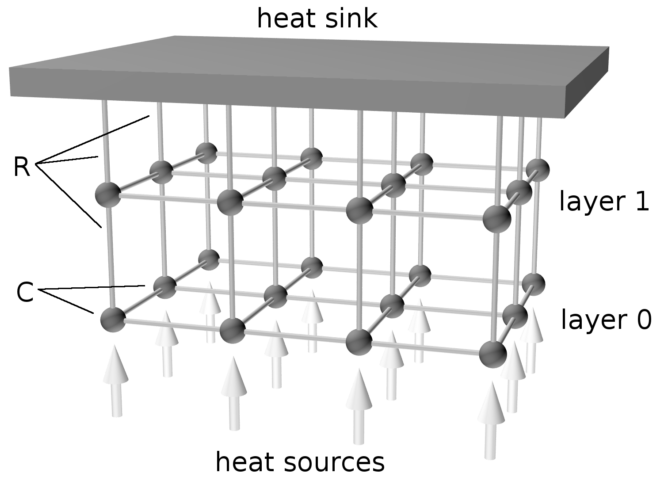
\includegraphics[scale=0.43]{figures/rcn}}
        \caption{RC-Network with two layers \cite{Happe}}
        \label{fig:rcn}
\end{figure}
 
\begin{figure}[ht]
        \center{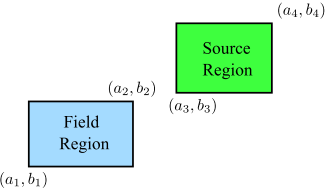
\includegraphics[scale=0.58]{figures/source_field_region}}
        \caption{The temperature in the field region is calculated from the power of the source field \cite{Sapatnekar2005}}
        \label{fig:fields}
\end{figure}
 
Another approach for post-fabrication heat flow modeling is proposed in \cite{Sapatnekar2005}.
Just as HotSpot, this approach requires knowledge about the chip's structure, the layers' thickness and thermal conductivity. However, it does not model the thermal behavior as an RC network. On the contrary, the temperature distribution in a field region located between the chip's coordinates $(a_1,b_1)$ and $(a_2,b_2)$ is derived from the power source located between $(a_3,b_3)$ and $(a_4,b_4)$. Figure~\ref{fig:fields} depicts these regions located on the chip.
 
This approach faces the problem of solving the heat diffusion equation, which is the differential equation
 
\begin{equation}
\label{eq:hde}
\rho c_p \frac{\partial T(x,y,z,t)}{\partial t} =
\nabla \cdot [k(x,y,z,T) \nabla T(x,y,z,t)] +g(x,y,z,t)
\end{equation}
 
where $\rho$ is the density of the material ($\frac{kg}{m^3}$), $c_p$ is the specific heat ($\frac{J}{kg\cdot ^\circ C}$), T is the temperature ($^\circ C$) , $k$ is the thermal conductivity ($\frac{W}{m \cdot ^\circ C}$), $g$ is the volume power density ($\frac{W}{m^3}$) and $(x,y,z)$ are the die's coordinates \cite{Sapatnekar2005}.
 
\section{Goals of the Thesis}
\label{sec:goals}
 
\subsection{On-Line Heat Flow Modeling Approach}
\label{sec:online}
 
In many application areas of today's VLSI the on-chip temperature prediction is becoming increasingly important. The heat flow modeling approaches at design time introduced in Section~\ref{sec:approach} are solely suitable devices where the internal chip structure is known. This does not apply to all devices. The on-line heat flow modeling approach is based on this problem.
In contrary to the post-fabrication heat flow modeling approaches, the on-line approach benefits from dropping the requirements of knowing the internal layer structure of a chip, such as heat conductivity. However, the proposed system \cite{Happe} also takes advantage of an RC network. But, for the sake of performance, the accuracy is slightly decreased in this model. That is, the number of layers is reduced to two, as Figure~\ref{fig:rcn} depicts. This trade-off reduces the complexity of the system in order to be executed efficiently on embedded devices. Furthermore, increasing the amount of layers only marginally improve the prediction, whereas a greater workload for the learning algorithm is generated.
 
The approach resorts to a black box heat and internal layer structure. The RC network's parameters are tuned online by a heuristic.
That is, instead of having fixed parameters for the thermal model, the on-line approach contains a set of free parameters $P$, which are initialized randomly at the beginning of the learning process and improved at each step $t_i$.
The improvement happens according to the deviation in the model's temperature prediction from the actual measured heat distribution.
Technically, the thermal model is improved by comparing the actual temperature of the die $T_m(t_i,i)$ and the predicted temperature $T_s(P,t_i,j)$ for each node $j$. The learning is done by randomized hill climbing in this approach. The goal is the minimization of the mean square error $mse$ dependent on the parameters $P$.
 
\begin{equation}
\label{eq:mse}
mse(P)=\frac{1}{|N||M|} \cdot \sum_{i\in M} \sum_{j\in N} (T_s(P,t_i,j)-T_m(t_i,j))^2
\end{equation}
 
 
\subsection{Thesis Objectives}
\label{sec:objectives}
 
As proposed above there are several ways to model heat flow on integrated devices.
The thesis gives an overview on heat models using physical device models and other post-fabrication approaches like the RC-network. Furthermore the on-line extension of these models, which were briefly introduced above, will be explained in detail.
 
The main goal of the thesis is to improve the on-line approach of generating a heat model. Improvements are required desirable, as the approach stated in \cite{Happe} only remains within a temperature range of $8^\circ$C with a average root mean square error of $0.72^\circ$C. The temperature range will be increased by creating higher temperature gradients by dint of \cite{Agne2013}. The average root mean square error is planned to be decreased by using evolutionary learning and optimizing algorithms.
Besides the general methodology all necessary approaches will be explained, like temperature generation and measurement and learning and optimizing algorithms, like Simulated Annealing and Evolutionary Algorithms. These are the parts where the improvement to existing approaches may occur. Learning and optimizing algorithms are used to redefine the model's set of parameters in order to achieve an efficient and precise heat model on-line. Each of these approaches will be tested and afterwards evaluated by discussing and comparing its effort for creating a the model and the accuracy of heat prediction. That is, the evolutionary approaches are measured based on the results obtained by the randomized hill climbing used in the approach stated in \cite{Happe}, which is efficiency and accuracy of prediction.
 
%After presenting the general methodology of improving the on-line approach several learning and optimizing algorithms are presented which may improve on-line heat models. Evolutionary Algorithms or Simulated Annealing are examples for a possible evolution. Improvement is achieved by efficiently set the model's parameters which allow precise temperature prediction.
 
 
%In order to enable that the temperature sensor grid including several heat-generating cores need to be implemented on the an Xilinx Virtex-5 FPGA (XUPV5-LX110T). In addition to that, there will be a host PC connected to the FPGA, which controls the experiments and adjusts the model's parameters.
 
%The main goal of the thesis is to improve the on-line prediction proposed in \cite{Happe}. With help of more efficient heat-generating cores, which were introduced in \cite{Agne2013}, the model shall be improved. Furthermore, the on-line learning algorithm used in the approach given in Section~\ref{sec:online} will be replaced by other algorithms, which might be more efficient, for example by Simulated Annealing or Evolutionary Algorithms. The result's quality will be evaluated by comparing it to conventional heat flow modeling approaches, which were briefly introduced above.
 
\section{Structure of the Thesis}
\label{sec:structure}
 
The thesis will be structured as follows:
 
\begin{itemize}
\item{\bf{Introduction}}
Introduction to heat modeling and the reason why it becomes eminent for new many-core and reconfigurable devices
 
\item{\bf{Heat Modeling of integrated Devices}}
\subitem{Heat Models using physical device models}
\subitem{Other Methods (e.\,g. RC-\,Networks)}
\subitem{Extension to On-Line Evolution of Heat Models}
\subitem{Temperature Generation Methods}
\subitem{Temperature Measurement Methods}
\subsubitem{Discussion on Accuracy}
\item{\bf{Online Evolution of Heat Models}}
\subitem{Methodology}
\subsubitem{Definition of Heat Model}
\subsubitem{Measurement modes and Accuracy}
\subitem{Learning and Optimizing Algorithms}
\subsubitem{Methodology of used Algorithms}
\item{\bf{Experiments and Evaluation}}
\subitem{Experiments on RC-network}
\subitem{Results for several Learning Algorithms}
\subitem{Discussion of Convergence}
\subitem{Discussion of Accuracy}
\subitem{Discussion of On-Line Suitability}
\subitem{Discussion of Embedded Implementation}
\item{\bf{Conclusion}}
 
%\item{\bf{Heat Flow Modeling Approaches}}
%\subitem{\bf{Post-Fabrication}}\\
%A detailed overview over post-fabrication heat flow approaches
%\subitem{\bf{On-Line}}\\
%Based on \cite{Happe}, the on-line approach is introduced in detail
%\item{\bf{Evolution of On-Line Heat Flow Modeling Approach}}
%\subitem{\bf{Learning Algorithms}}\\
%Different learning algorithms are introduced in this section
%\subitem{\bf{Methodology}}\\
%Methodology and experimental design of the evolutionary on-line learning algorithm
%\item{\bf{Evaluation}}
%The thermal model is evaluated by comparison with conventional temperature models
%\item{\bf{Conclusion}}
\end{itemize}
 
\section{Time Schedule}
\label{sec:time}
 
Figure~\ref{fig:schedule} depicts the intended time schedule of the thesis.
 
\begin{figure}[!ht]
        \center{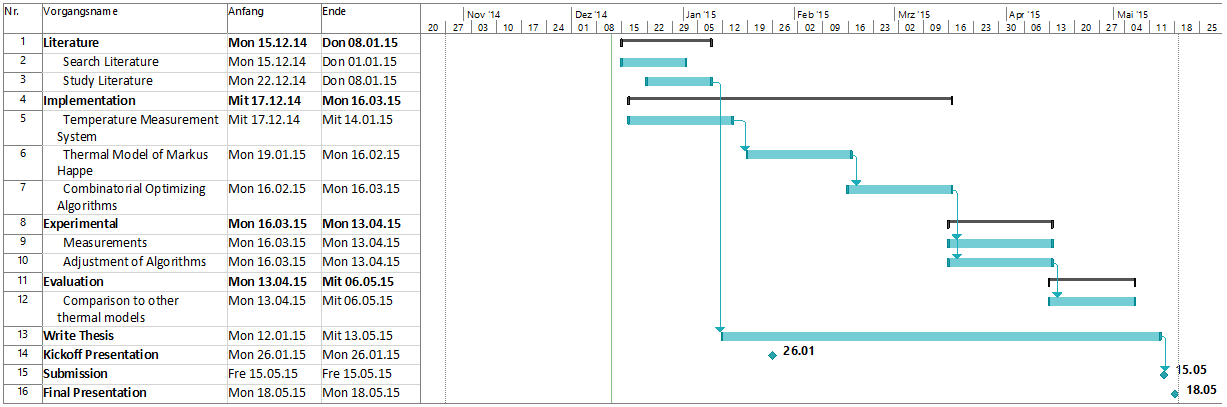
\includegraphics[angle=270, scale=0.59]{figures/time_sched.png}}
        \caption{Time schedule}
        \label{fig:schedule}
\end{figure}
 
 
\section{Thesis Organization}
\label{sec:orga}
Besides the thesis' contents, there are several organizational tasks which will be performed during the thesis.
\begin{itemize}
\item{\bf Kick-Off Presentation}
The thesis' topic and time schedule will be introduced in a 15 minutes presentation.
 
\item{\bf Frequent Meetings}
Every (second) week there will be a meeting with the supervisor, in order to keep track of the thesis' progress and potential issues.
 
\item{\bf Documentation}
The thesis will be documented accurately. Care is given to clarity and completeness.
 
\item{\bf Final Presentation}
Referring to the target agreement, the obtained results will be presented after the submission of the thesis.
 
\item{\bf Submission}
The complete compilable and synthesizable code, experimental data, slides of both presentation and the thesis itself will be submitted in digital form.
\end{itemize}
 
\bibliography{bib}
\bibliographystyle{plain}
 
\end{document}